%In the previous section \ref{NN}, we have seen, that an artificial neuron maps input data to an output signal as $y=\sigma(W\cdot x+b)$.
%The simplest neural network would just be the linear operation $W\cdot x+b$.
%But if we use an activation function, we result on the one hand different slopes on the output functions. 
%On the other hand its function at the network's last layer is to focus the outputs of the previous linear operation inside a specified range.

%In the following we will discuss as Stevens et al. \cite{antiga_deep_2020} did, some different activation functions like the Heaviside's Threshold Function, \ac{RELU}, Sigmoid-Function or Tangens Hyperbolicus, which are visualized in figure \ref{fig:actFunc}.
%In the previous section (Section \ref{NN}), we saw that an artificial neuron maps an input vector $s\in \mathbb{R}^n$ to an output via the equation
%\[y = \sigma(w^\top x +b),\]
%where $w\in \mathbb{R}^n$ is a weight vector, $b\in \mathbb{R}$ is a bias term, and $\sigma$ is a non-linear activation function.

%Extending this to a fully layer with $m$ neurons, the model computes 
%\[y = \sigma(Wx+b),\]
%where $W\in \mathbb{R}^{m\times n}, b \in \mathbb{R}^m$ and $\sigma$ is applied element-wise.
In the previous section (Section \ref{NN}), we saw that a model  a fully connected layer computes outputs via the quation: \[y = \sigma(Wx+b),\] 
where $W\in \mathbb{R}^{m\times n}$ is the weight matrix, $b\in \mathbb{R}^m$ is a bias vector, and $\sigma$ is a non-linear activation function.



%If we don't consider the activation function, we only have an affine transformation  $Wx+b$, the model becomes purely linear.
%While such models are useful in simple settings (e.g. linear regression), they are limited in ther expressive power.
%A composition of linear functions is still linear, which means that even deep networks without non-linearities cannot represent complex patterns or decision boundaries. 

%The inclusion of non-linear activation functions is what gives neural networks the ability to approximate a wide class of functions, including any continuous function on a compact domain. %As shown in the Universal approximation theorem

If we don't consider the activation function, we only have an affine transformation  $Wx+b$, resulting in a purely linear model.While such models are useful in simple settings (e.g. linear regression), they are limited in ther expressive power.
A composition of linear functions is still linear, which means that even deep networks without non-linearities cannot represent complex patterns or decision boundaries. 

The inclusion of non-linear activation functions, particularly continuous sigmoidal functions endows neural networks with the expressive capacity to approximate a wide range of functions.
In fact, the Universal Approximation Theorem states that a feedforward neural network with a single hidden layer and a continuous sigmoidal activation function can uniformly approximate any continuous function defined on a compact domain, such as the unit hypercube $[0,1]^n$ \cite{cybenkot_approximation_nodate}.

Activation functions define the function space that a neural network can represent.
Their properties influence not only the expressive capacity of the network, but also its trainability, optimization dynamics, and numerical stability.

In the following, we discuss several commonly used activation functions as presented in Stevens et al. \cite{antiga_deep_2020}, including Heaviside's threshold function, the Rectified Linear Unit (ReLU), the sigmoid function, and the hyperbolic tangent. These functions are illustrated in Figure~ \ref{fig:actFunc}.

\begin{enumerate}
    \item[(a)] \textbf{Heaviside function}
    \begin{itemize}
        \item is a historically significant choice of activation function
        \item $\sigma(x) = H(x) :=
            \begin{cases} 
              0, & x < 0 \\
              1, & x \geq 0
            \end{cases}$
    \end{itemize}
    \item [(b)] \textbf{\ac{RELU}}
    \begin{itemize}
        \item one of the most used activation function in modern neural networks
        \item $\sigma(x)=\text{ReLU}(x):=\max\{0,x\}$
    \end{itemize}
    \item [(c)] \textbf{Sigmoid}
    \begin{itemize}
        \item commonly used activation function in early neural networks
        \item reason that activation functions are often labelled with $\sigma$
        \item $\sigma(x)=\text{Sigmoid}(x):=\frac{1}{1+e^{-x}}$
    \end{itemize}
    \item [(d)] \textbf{Hyperbolic tangent}
    \begin{itemize}
        \item similar to the sigmoid 
        \item $\sigma(x) = \tanh(x):=\frac{e^x-e^{-x}}{e^x+e^{-x}}$
    \end{itemize}
\end{enumerate}
\begin{figure}[h]
    \centering
    % Heaviside-Funktion
    \begin{subfigure}{0.24\textwidth}
        \centering
        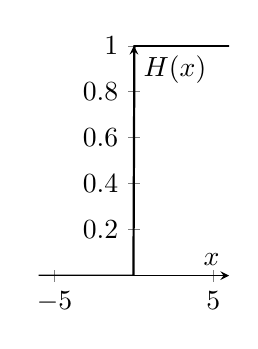
\begin{tikzpicture}
            \begin{axis}[
                axis lines = middle,
                xlabel = $x$, ylabel = $H(x)$,
                width=4cm, height=4.5cm
            ]
            \addplot[black, thick, domain=-6:6, samples=200] {x >= 0 ? 1 : 0};
            \end{axis}
        \end{tikzpicture}
        \caption{Heaviside}
    \end{subfigure}
    \hfill
    % ReLU-Funktion
    \begin{subfigure}{0.24\textwidth}
        \centering
        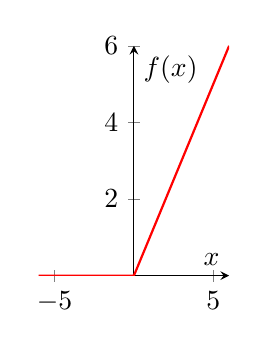
\begin{tikzpicture}
            \begin{axis}[
                axis lines = middle,
                xlabel = $x$, ylabel = $f(x)$,
                width=4cm, height=4.5cm
            ]
            \addplot[red, thick, domain=-6:6, samples=200] {max(0, x)};
            \end{axis}
        \end{tikzpicture}
        \caption{ReLU}
    \end{subfigure}
    \hfill
    % Sigmoid-Funktion
    \begin{subfigure}{0.24\textwidth}
        \centering
        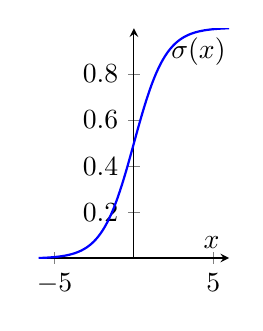
\begin{tikzpicture}
            \begin{axis}[
                axis lines = middle,
                xlabel = $x$, ylabel = $\quad \sigma(x)$,
                width=4cm, height=4.5cm
            ]
            \addplot[blue, thick, domain=-6:6, samples=200] {1 / (1 + exp(-x))};
            \end{axis}
        \end{tikzpicture}
        \caption{Sigmoid}
    \end{subfigure}
    \hfill
    % Tanh-Funktion
    \begin{subfigure}{0.24\textwidth}
        \centering
        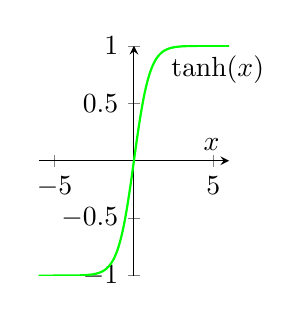
\begin{tikzpicture}
            \begin{axis}[
                axis lines = middle,
                xlabel = $x$, ylabel = $\quad\tanh(x)$,
                width=4cm, height=4.5cm
            ]
            \addplot[green, thick, domain=-6:6, samples=200] {tanh(x)};
            \end{axis}
        \end{tikzpicture}
        \caption{Tanh}
    \end{subfigure}
    \caption{Activation functions}
    \label{fig:actFunc}
\end{figure}

\newpage

There exists some common multivariate functions as Softmax and Maxpool, too.
His multivariate functions operate on vectors and tensor and are commonly used to transform a vector of real-values scores into a probability distribution over classes. 
\begin{enumerate}
    \item[(a)] \textbf{Softmax}
    \begin{itemize}
        \item For \( \lambda > 0 \), the scaled softmax is defined as
        \[
            \operatorname{softmax}_\lambda: \mathbb{R}^n \to [0,1]^n,\quad 
            \operatorname{softmax}_\lambda(x)_i = \frac{e^{\lambda x_i}}{\sum\limits_{j=1}^{n} e^{\lambda x_j}},\quad \forall i \in \{1, \dots, n\}.
        \]
    \end{itemize}
	\item[(b)] \textbf{Maxpool operation}
	\begin{itemize}
		\item The maxpool function is defined as
		\[
		\operatorname{maxpool}: \mathbb{R}^n \to \mathbb{R}^m, \qquad 
		\operatorname{maxpool}(x)_i = \max_{j \in I_i} x_j 
		\quad \text{for all } i \in \{1, \dots, m\},
		\]
		where \( I_i \subset \{1, \dots, n\} \) defines the pooling region.
	\end{itemize}
\end{enumerate}


\subsection{Training Process}
After introducing layers and non-linear activation functions, we now have all required components for a neural network to approximate complex functions.
However, in order to fit an actually given task such as mapping inputs to outputs, we shall need to determine appropriate values for the networks weights and biases.
This is where we use the trainings process. 
The goal of training process is to adjust the parameters of a neural network that explains the best relationship between the given inputs and outputs.
This is achieved by computing the error between the networks output and the target values using a loss function $\mathcal{L}$ and then propagating this error backwards through the network to update the parameters, this process is known as backpropagation. 
During backpropagation, the network applies the chain rule to pass the error from the output layer back to the earlier layers, adjusting weights and biases along the way in order to minimize the loss.



A loss function \(\mathcal{L}\) measures the discrepancy between the network's predicted output and the true target value.  
Its purpose is to guide the training process by quantifying how wrong the network's predictions are.

It measures the  loss of the model and will be minimized during the training process.
Common choices of loss functions, as presented in \cite{zhou_machine_2021}, include:
%Therefore, the model adjusts the weights using different approaches, like squared error loss or cross entropy, as presented in \cite{zhou_machine_2021}.

\begin{enumerate}
    \item[(a)] \textbf{Squared Error Loss}
    \begin{itemize}
        \item Measures the squared difference between predicted and target values.
        \item Often used in regression settings, but can also be applied to compare continuous representations in higher-dimensional spaces.
        \item Defined as
        \[
        \mathcal{L}_{\operatorname{SquareErr}}(y, \hat{y}) = \sum_{i = 1}^{n} \| y_i - \hat{y}_i \|^2.
        \]
    \end{itemize}
    
    \item[(b)] \textbf{Cross Entropy Loss}
    \begin{itemize}
        \item Used for classification tasks involving discrete probability distributions.
        \item Let $p = (p_1, \dots, p_k)$ and $q = (q_1, \dots, q_k)$ be discrete probability distributions over $k$ classes.
        \item Defined as
        \[
        \mathcal{L}_{\operatorname{CrossEnt}}(p, q) = -\sum_{i=1}^{k} p_i \ln q_i.
        \]
    \end{itemize}
    
    \item[(c)] \textbf{Huber Loss}
    \begin{itemize}
        \item Combines properties of squared error loss and absolute error loss..
        \item Less sensitive to outliers than squared error loss.
        \item Introduced by Peter J. Huber in his foundational work on robust statistics \cite{gokcesu2021generalizedhuberlossrobust}
        \item Defined for a threshold $\delta > 0$ as
        \[
        \mathcal{L}_{\operatorname{Huber}}(y, \hat{y}) =
        \sum_{i=1}^{n}
        \begin{cases}
            \frac{1}{2} (y_i - \hat{y}_i)^2 & \text{if } |y_i - \hat{y}_i| \leq \delta, \\
            \delta \left( |y_i - \hat{y}_i| - \frac{1}{2} \delta \right) & \text{otherwise}.
        \end{cases}
        \]
    \end{itemize}
\end{enumerate}


We now formalize the training task. 
Let $\mathcal{D} := \{(x_i, y_i)\}_{i=1}^n$ be a dataset of input-output pairs, where $x_i$ are the inputs and $y_i$ the corresponding labels.  
Let $f(x, \theta)$ be a neural network parameterized by $\theta$ that maps inputs to outputs.  
We define the set of all trainable parameters, i.e., the weight matrices and bias vectors of each layer $l = 1,\dots,L$, as
\[
\theta := \{(W^{(l)}, b^{(l)}) \mid W^{(l)} \in \mathbb{R}^{m_l \times n_l},\ b^{(l)} \in \mathbb{R}^{m_l} \}.
\]

Following Smets~\cite{smets2024mathematicsneuralnetworkslecture}, we define the sample-wise loss as
\[
\tilde{f}_i(\theta) := \mathcal{L}(y_i, f(x_i, \theta)) \quad \text{for } i = 1, \dots, n,
\]
and define the overall training objective as minimizing the average loss across the dataset:
\[
\min_{\theta} \frac{1}{n} \sum_{i=1}^{n} \tilde{f}_i(\theta).
\]

To solve this optimization problem, gradient-based methods such as \emph{stochastic gradient descent} (SGD) are commonly used.  
These methods update the model parameters iteratively in the direction that reduces the loss.

Concretely, the parameters \(\theta\) are updated via the rule
\[
\theta \leftarrow \theta - \eta \cdot \nabla_\theta \left( \frac{1}{n} \sum_{i=1}^{n} \tilde{f}_i(\theta) \right),
\]
where \(\eta > 0\) is the learning rate that controls the step size.  
The required gradients \(\nabla_\theta \mathcal{L}(y_i, f(x_i, \theta))\) are efficiently computed using \emph{backpropagation}, which applies the chain rule to propagate derivatives through the network layers.
In classical \emph{gradient descent}, the full gradient over the entire dataset is used in each step. 
This becomes computationally expensive for large datasets.
In contrast, \emph{stochastic gradient descent (SGD)} approximates this full gradient by computing it on small random subsets of the data, called mini-batches.
This introduces some noise into the updates but allows for faster and more scalable training.

One widely used variant of SGD is the \emph{Adam optimizer} \cite{kingma2017adammethodstochasticoptimization}, which adaptively adjusts the learning rate for each parameter based on estimates of the first and second moments of the gradients.
Adam combines the benefits of two earlier methods, and often leads to faster convergence and more stable training, especially in deep networks.



The following code snippet~\ref{lst:train-func} shows the training routine of a neural network used to learn a nonlinear transformation for intrinsic homotopy, which will be discussed in detail in Chapter~\ref{ISA}.
\lstinputlisting[
  caption={Code snippet showing how to train a neural network},
  label={lst:train-func},
   basicstyle=\small\ttfamily,
  firstline=1,
  lastline=55
]{Abschlussarbeit/Text/NeuralNetwork/train_NN_.py}


